\documentclass[11pt,a4paper]{article}
\usepackage[margin=2.4cm]{geometry}
\usepackage{amsmath,amssymb,booktabs,graphicx,xcolor,microtype}
\usepackage[colorlinks=true,linkcolor=blue!45!black,urlcolor=blue!45!black]{hyperref}
\usepackage{titlesec}
\titleformat{\section}{\large\bfseries}{\thesection.}{0.6em}{}
\titleformat{\subsection}{\normalsize\bfseries}{\thesubsection}{0.6em}{}
\setlength{\parskip}{0.45em}\setlength{\parindent}{0pt}
\newcommand{\code}[1]{\texttt{\small #1}}
\newcommand{\vn}{v_n}
\newcommand{\bsub}{\beta_{\mathrm{sub0}}}
\newcommand{\dsub}{d_{0,\mathrm{sub0}}}
\newcommand{\tsub}{\tau_{\mathrm{sub}}}

\title{\vspace{-1.4cm}\textbf{The sublimation kinetic coefficient was inflated by an\\
inapplicable thin-interface correction}\\
\large What was wrong, how it was found, what was changed, and why it works}
\author{\normalsize \code{lunar\_regolith\_DSM} and \code{enceladus\_DSM}}
\date{\normalsize 2026-09-09}

\begin{document}\maketitle\vspace{-0.7cm}

\begin{center}\fbox{\parbox{0.94\textwidth}{\small
\textbf{Summary.} The solver did not deliver the attachment kinetics it was given.
$\tsub$, the phase-field relaxation time, carried two Karma thin-interface counter-terms
intended to cancel a spurious contribution generated at finite interface width. For this
model that contribution is zero, because vapor diffuses only in the pore, so nothing
cancelled and the realized kinetic coefficient came out as $\bsub+\Delta$ instead of
$\bsub$. At $-20\,^\circ$C with $\epsilon=8.58\times10^{-7}$\,m the excess $\Delta$ was
$22\,\%$, and because $\Delta$ is proportional to $\epsilon$ the realized kinetics
depended on the mesh. The defect was found by fitting the Gibbs--Thomson relation
directly to nine wedge-channel runs, which recovered the capillary length exactly but
put the kinetic coefficient $22\,\%$ high; it was confirmed by a sweep in $\bsub$ over a
range of $40$, which reproduced the predicted shortfall from $0.32$ to $0.95$. The fix is
to remove the two terms (\code{-thin\_iface\_corr}, default $0$). After it, five runs
spanning the same range recover the requested kinetics to within $1\,\%$, and a
mirror-image control reproduces both menisci to $0.1\,\%$. One check remains outstanding:
that the answer no longer moves when $\epsilon$ is refined.}}\end{center}

\section{What the solver is supposed to do}

The model advances an ice phase field $\phi$ ($1$ in ice, $0$ in vapor) coupled to a
vapor density $\rho_v$. At the ice--vapor interface it is intended to satisfy the
Gibbs--Thomson condition
\begin{equation}
\sigma \;=\; \bsub\,\vn \;+\; \dsub\,\chi ,
\qquad
\sigma=\frac{\rho_v-\rho_{vs}(T)}{\rho_{vs}(T)} ,
\label{eq:gt}
\end{equation}
in which $\sigma$ is the supersaturation, $\rho_{vs}(T)$ the saturation vapor density,
$\vn$ the interface normal velocity (positive for growth), and $\chi$ the sum of the
principal curvatures (positive where the ice is convex into the vapor). The two
coefficients are user inputs: \code{-beta\_sub0}, the attachment kinetic coefficient,
which is set from the condensation coefficient $\alpha_c$ through the Hertz--Knudsen
relation $\bsub\propto1/\alpha_c$; and \code{-d0\_sub0}, the capillary length, set by the
ice surface energy. Equation~\eqref{eq:gt} is the target physics and is not in question
anywhere in this note.

The phase-field equation that is supposed to produce Eq.~\eqref{eq:gt} is
\begin{equation}
\tsub\,\partial_t\phi=\epsilon^2\nabla^2\phi-f'(\phi)
+\lambda_{\rm sub}\,g(\phi)\,\frac{\rho_{vs}(T)}{\rho_{\rm ice}}\,\sigma ,
\label{eq:pf}
\end{equation}
where $\epsilon$ is the interface parameter, $f$ the double well, $g(\phi)=\phi^2(1-\phi)^2$
the coupling function, and $\lambda_{\rm sub}$ and $\tsub$ are chosen so that the
sharp-interface limit of Eq.~\eqref{eq:pf} reproduces Eq.~\eqref{eq:gt} with the requested
$\dsub$ and $\bsub$.

\section{What was wrong}

\subsection{The counter-terms}
Taking $\epsilon\to0$ in Eq.~\eqref{eq:pf} gives Eq.~\eqref{eq:gt} with
\begin{equation}
d_{0,\rm realized}=\dsub,\qquad
\beta_{\rm realized}=\frac{\tsub\,\dsub}{\epsilon^{2}}-C_{\rm corr} .
\label{eq:limit}
\end{equation}
$C_{\rm corr}$ is a \emph{spurious} $O(\epsilon)$ term: at any finite interface width
$\sigma$ varies across the interfacial region where the phase change happens, and that
variation feeds back through the $\lambda_{\rm sub}g(\phi)\sigma$ coupling to add an
unwanted kinetic contribution. The standard remedy, due to Karma \& Rappel
(Phys.\ Rev.\ E \textbf{57}, 4323, 1998), is to inflate $\tsub$ by exactly the expected
$C_{\rm corr}$ so that the two cancel in Eq.~\eqref{eq:limit}. The solver did this:
\begin{equation}
\tsub=\epsilon\lambda_{\rm sub}\Big(
\underbrace{\tfrac{\beta_{\rm sub}}{a_1}}_{\text{the kinetics requested}}
+\underbrace{\tfrac{a_2\epsilon}{\texttt{diff\_sub}}}_{\text{thermal counter-term}}
+\underbrace{\tfrac{a_2\epsilon}{\texttt{dif\_vap}}}_{\text{vapor counter-term}}\Big),
\label{eq:tau}
\end{equation}
with $a_1=5$ and $a_2=0.1581$ the constants for this model's double well,
\code{diff\_sub} the mean thermal diffusivity and \code{dif\_vap} the vapor diffusivity.
The bracket is written in the $\rho_{vs}/\rho_{\rm ice}$-scaled variables the solver
carries internally.

\subsection{The consequence}
If $C_{\rm corr}$ is not in fact produced, nothing cancels, the inflation survives, and
the realized coefficient is
\begin{equation}
\beta_{\rm realized}=\bsub+\Delta,
\qquad
\Delta = a_1a_2\,\epsilon\left(\frac{1}{\texttt{diff\_sub}}+\frac{1}{\texttt{dif\_vap}}\right)
\frac{\rho_{\rm ice}}{\rho_{vs}(T)} .
\label{eq:delta}
\end{equation}
$\Delta$ is the central quantity of this note: the excess kinetic coefficient, in the
same units as $\bsub$ (s\,m$^{-1}$). At $-20\,^\circ$C with $\epsilon=8.584\times10^{-7}$\,m
it is $1.282\times10^{5}$\,s\,m$^{-1}$, against a requested
$\bsub=5.9216\times10^{5}$: an excess of $22\,\%$, of which three quarters comes from the
thermal term.

\section{How it was found}

\subsection{Measurement}
The wedge geometry places an apex-centered ice annulus in a tapering pore, with the
virtual apex on the channel axis. On the centerline the interface normal is therefore
exactly $\pm\hat x$ and $\vn$ reduces to a one-dimensional displacement rate, which makes
it measurable without reconstructing normals or differentiating contours.
\code{postprocess/wedge\_gt\_velocity.py} measures $\sigma$, $\chi$ and $\vn$ on both
menisci of each run.

\subsection{Fitting both coefficients}
Rather than assume Eq.~\eqref{eq:gt} and report a ratio, both coefficients were fitted.
Each snapshot gives a triple $(\sigma,\vn,\chi)$, so
$\sigma=\beta\vn+d_0\chi$ is a two-column least-squares problem. It is identifiable
because the two menisci carry curvature of opposite sign, the inner being concave and the
outer convex, while a $3\times3$ grid of vapor boundary conditions varies $\vn$ at nearly
fixed $\chi$ (condition number $2.58$). Over nine runs, $n=3492$:
\begin{center}\small\begin{tabular}{lrr}\toprule
 & fitted & relative to requested\\ \midrule
$d_0$   & $1.0172\times10^{-9}$\,m       & $1.0006$\\
$\beta$ & $7.2324\times10^{5}$\,s\,m$^{-1}$ & $1.2214$\\ \bottomrule
\end{tabular}\end{center}
with $R^2=0.999997$ and an rms residual of $0.14\,\%$ of $|\sigma|$. Two things follow.
The relation itself holds: a different functional form would not fit this well. And the
capillary length is delivered exactly, so the discrepancy is confined to $\beta$. Since
$\beta$ and $d_0$ are separately identified, they are not trading off; $d_0$ came out
correct both before and after the fix, while $\beta$ moved by $22\,\%$.

The fitted $\beta$ agrees with Eq.~\eqref{eq:delta} to $0.4\,\%$, which identifies the
counter-terms as the source.

\subsection{Confirming it}
Because $\Delta$ is additive and does not scale with $\bsub$, the predicted shortfall
$\bsub/(\bsub+\Delta)$ is a strong function of $\bsub$. Four runs differing only in
\code{-beta\_sub0}, each 3406 steps (batch \code{2026-08-25\_\_18.14.15\_beta\_ladder}):
\begin{center}\small\begin{tabular}{rrrrr}\toprule
$\bsub$ relative & predicted & \multicolumn{2}{c}{measured} & $\beta_{\rm fit}/(\bsub+\Delta)$\\
 & ratio & inner & outer & \\ \midrule
$0.10\times$ & 0.3160 & 0.3239 & 0.3082 & 1.0004\\
$0.25\times$ & 0.5359 & 0.5444 & 0.5254 & 1.0015\\
$1.00\times$ & 0.8220 & 0.8253 & 0.8126 & 1.0017\\
$4.00\times$ & 0.9487 & 0.9471 & 0.9429 & 1.0000\\ \bottomrule
\end{tabular}\end{center}
The ratio moves by a factor of $2.9$ and follows the prediction to $2.3\,\%$. A constant
$1.00$, meaning the counter-terms work as intended, and a constant $0.82$, meaning a fixed
factor of some other origin, are both excluded by every run. Fitting $\beta$ with $d_0$
held fixed gives $\beta_{\rm fit}/(\bsub+\Delta)=1.0009\pm0.0007$, so $C_{\rm corr}=0$ to
better than one part in $10^3$.

\section{Why the correction is absent}

The Karma \& Rappel counter-term is derived for a \emph{symmetric} model, meaning the
diffusing quantity has the same diffusivity in both phases. Our vapor equation instead
carries $D_v\phi_a$, where $\phi_a=1-\phi$: vapor diffuses in the pore and not in the ice.
This is the \emph{one-sided} case, and it behaves differently.

Write $\zeta$ for signed normal distance from the interface and $\eta=\zeta/\epsilon$ for
the stretched inner coordinate. Expanding $\phi=\phi_0(\eta)+\epsilon\phi_1+O(\epsilon^2)$,
where the subscript is the order in $\epsilon$ and not a phase label, the leading term
$\phi_0=\tfrac12(1+\tanh(\eta/2))$ is the planar equilibrium profile. Splitting
$\sigma=\sigma_{\rm int}+\delta\sigma(\eta)$, with $\sigma_{\rm int}$ the outer solution
extrapolated to the interface, the counter-term is proportional to
\begin{equation}
I=\int g(\phi_0)\,\partial_\eta\phi_0\;\delta\sigma(\eta)\,\mathrm{d}\eta .
\label{eq:I}
\end{equation}
Neglecting storage, which is smaller than diffusion by $2.4\times10^{-11}$ here, the inner
vapor balance integrates once to
\begin{equation}
D_v\phi_a\,\partial_\eta\rho_v=\epsilon \vn\rho_{\rm ice}\,\phi_a
\;\;\Longrightarrow\;\;
\partial_\eta\rho_v=\frac{\epsilon \vn\rho_{\rm ice}}{D_v}
\quad\text{wherever }\phi_a\neq0 ,
\end{equation}
the constant of integration being fixed by the absence of flux into the ice. The factor
$\phi_a$ cancels, and the surviving constant is exactly the outer Stefan gradient. The
inner solution is therefore the outer solution continued through the interface,
$\delta\sigma\equiv0$, and $I$ vanishes for any weight. With a symmetric $D$ the $\phi_a$
does not cancel, $\delta\sigma$ is non-zero and even in $\eta$, and $I$ survives; this is
the case Karma \& Rappel treat.

Two remarks. First, the thermal counter-term fails for an unrelated reason:
\code{a2*eps/diff\_sub} treats latent heat as driving $\sigma$ at unit strength, whereas
temperature reaches $\sigma$ only through $\rho_{vs}(T)$ and so carries a
Clausius--Clapeyron factor. The correct coefficient,
$(\mathrm{d}\rho_{vs}/\mathrm{d}T)L_{\rm sub}/k$, is smaller by a factor of $11$ to
$1300$. Second, the argument above bounds only the terms proportional to $\vn$. A
one-sided model without an anti-trapping current can also produce a spurious surface
diffusion, which is a different operator and is not observable in this measurement; see
\S\ref{sec:open}.

\begin{figure}[t]\centering
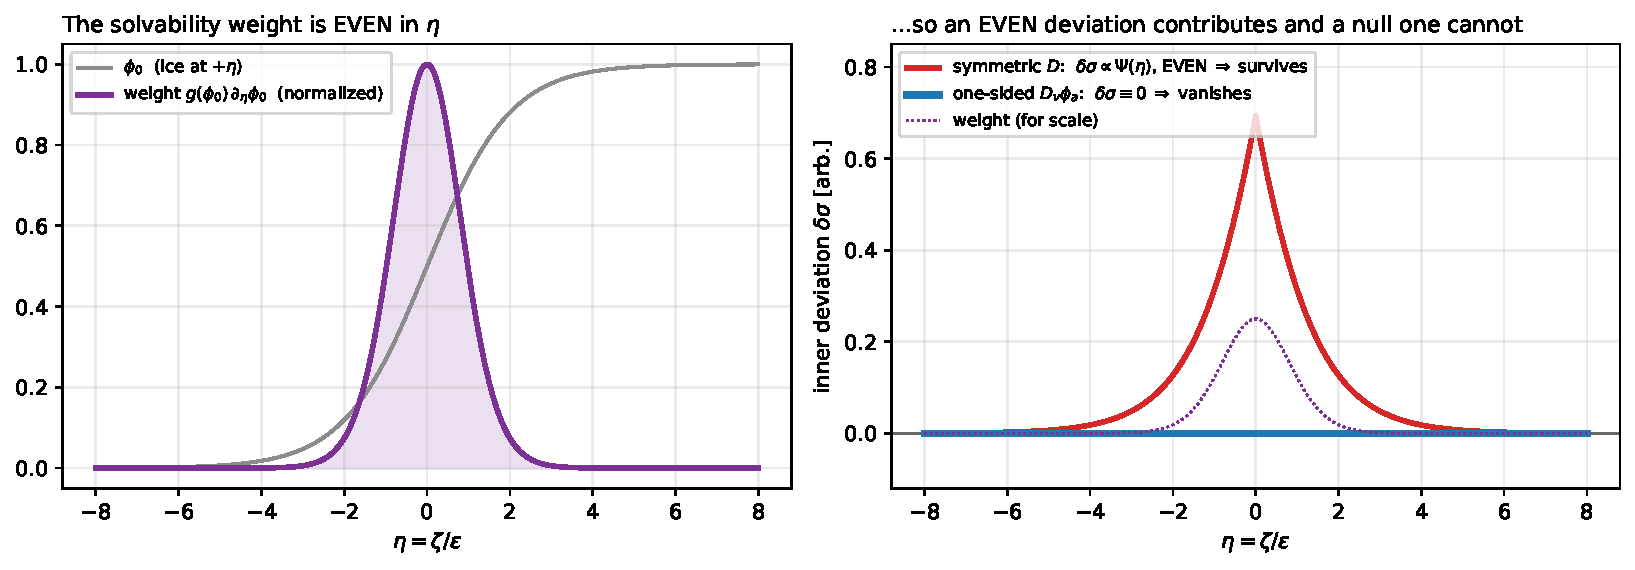
\includegraphics[width=\textwidth]{fig_inner.pdf}
\caption{\small Left: the weight $g(\phi_0)\,\partial_\eta\phi_0$ in Eq.~\eqref{eq:I} is
even in $\eta$. Right: with symmetric $D$ the inner deviation $\delta\sigma$ is even and
non-zero and the counter-term survives; with the one-sided $D_v\phi_a$ it vanishes
identically, so no counter-term can arise.}
\end{figure}

\section{The change}

Both counter-terms are now behind \code{-thin\_iface\_corr}, which defaults to $0$, in
the scalar path of both solvers and in the pointwise path \code{SubKinetics}, with the
analytic Jacobian derivatives gated alongside them. Setting the flag to $1$ restores the
terms in their historical form for comparison with earlier runs; it is not a corrected
form, and since the physically correct counter-term for this model is approximately zero,
no corrected form is provided. Each run now reports the realized coefficient in its
header.

Removing the terms is equivalent to supplying $\bsub-\Delta$ in their presence, but is
preferable: it is applied once rather than in every run configuration, cannot be
invalidated by a later change of $\epsilon$ or $T$, and remains defined when
$\Delta>\bsub$, where no pre-compensation exists. Rescaling $\bsub$ by the observed ratio
would not work at all, since that ratio is $\bsub/(\bsub+\Delta)$ and varies from $0.32$
to $0.95$ over the range tested.

\section{That the fix works}

Five runs, batch \code{2026-09-09\_\_09.22.56\_tau\_fix}, with no solver failures:
\begin{center}\small\begin{tabular}{lrrrl}\toprule
run & before & \multicolumn{2}{c}{after} & $\sigma$ sensitivity\\
 & & inner & outer & \\ \midrule
$0.10\times$ & 0.3160 & 1.0863 & 0.9539 & $9.5\,\%$ / $3.3\,\%$\\
$0.25\times$ & 0.5359 & 1.0330 & 0.9720 & $3.6\,\%$ / $1.4\,\%$\\
$1.00\times$ & 0.8220 & 1.0056 & 0.9877 & $0.9\,\%$ / $0.3\,\%$\\
$4.00\times$ & 0.9487 & 0.9985 & 0.9936 & $0.2\,\%$ / $0.1\,\%$\\ \bottomrule
\end{tabular}\end{center}
Fitting $\beta$ with $d_0$ held fixed gives $\beta_{\rm fit}/\bsub$ of $0.9916$, $1.0012$,
$1.0017$ and $1.0003$. The residual scatter tracks the last column run for run and is
therefore measurement rather than model. It is larger at small $\bsub$ for a physical
reason: with the correct, smaller $\beta$ the interface sits nearer local equilibrium, so
the residual $\sigma-\dsub\chi$ shrinks and a fixed absolute error in $\sigma$ becomes a
larger fraction of it. Precision is now best at large $\bsub$, the reverse of before.

\textbf{Mirror control.} A fifth run reflects the channel about $x=L_x/2$, putting the
wide end at $x=0$ and exchanging the two vapor reservoirs with it, so that the concave
meniscus moves from the left of the ice to the right. The two menisci exchange values
exactly:
\begin{center}\small\begin{tabular}{lrr}\toprule
 & inner (concave) & outer (convex)\\ \midrule
unmirrored & 1.0056 & 0.9877\\
mirrored   & 1.0056 & 0.9869\\ \bottomrule
\end{tabular}\end{center}
with $\dsub\chi$ agreeing to $0.07\,\%$. The residual $1\,\%$ difference between the two
menisci therefore follows the geometry rather than the side, and is a property of
curvature rather than an artifact of the mesh or the measurement.

\section{How this changes the model's behavior}\label{sec:effects}

The change alters the relationship between what is requested and what is realized. Every
statement below concerns the \emph{old} behavior; after the change the realized
coefficient is $\bsub$ and none of these dependencies remain.

\textbf{Attachment coefficient $\alpha_c$.} Since $\bsub\propto1/\alpha_c$ while $\Delta$
does not depend on $\alpha_c$ at all, the realized $\alpha_c$ was always lower than
requested, and increasingly so as $\alpha_c$ was raised. Worse, $\beta_{\rm realized}\ge\Delta$
placed a ceiling on the attainable $\alpha_c$ that no input could exceed. At
$\epsilon=8.584\times10^{-7}$\,m that ceiling was $0.062$ at $-20\,^\circ$C and $0.0006$
at $-60\,^\circ$C. Tuning $\alpha_c$ against experiment was therefore adjusting a knob
that did not do what it said, and hardest to move where the physics most wanted it moved.

\textbf{Interface parameter $\epsilon$.} $\Delta\propto\epsilon$, so the realized kinetics
depended on the mesh. This is the most serious consequence: a converged sharp-interface
limit cannot depend on $\epsilon$, so no mesh refinement could ever have converged.
Halving $\epsilon$ would have moved the ratio from $0.822$ to $0.902$.

\textbf{Diffusivities.} $\Delta\propto1/\texttt{diff\_sub}+1/\texttt{dif\_vap}$, so
raising either reduced the error. This matters for the Molaro study, where the
$D_v\times10$ arm was chosen to suppress transport resistance: because the thermal term
dominates $\Delta$ and does not involve $D_v$, that arm concentrated the error instead of
diluting it, and its rate loss was $10.7\,\%$ against $4.2\,\%$ for the nominal-$D_v$ arm.

\textbf{Temperature.} $\Delta\propto1/\rho_{vs}(T)$, so the error grew rapidly as
temperature fell: $22\,\%$ at $-20\,^\circ$C, a factor of $1.7$ at $-40\,^\circ$C, and a
factor of $20.7$ at $-60\,^\circ$C.

\textbf{What is unaffected.} Scaling exponents and dimensionless ratios, since they do not
depend on the absolute rate. Quantities that do depend on it, such as times to a given
state or absolute growth rates, are displaced by $\bsub/(\bsub+\Delta)$ for the
$(\epsilon,T,\alpha_c)$ of the run in question, and any earlier conclusion resting on one
should be re-checked. \code{preprocess/comp\_eps.py} sizes $\epsilon$ using $\bsub$; with
the counter-terms gone that relation is no longer implicit.

\section{Outstanding}\label{sec:open}

\textbf{$\epsilon$-convergence, staged and not yet run.} All of the above appeals to our
own analysis at some point. The one check that does not is refinement: a converged
sharp-interface limit cannot depend on $\epsilon$. \code{tests\_eps\_convergence.txt}
halves $\epsilon$ to $4.292\times10^{-7}$\,m ($989\times659$, four times the cells) and
predicts the same ratio as the existing $\epsilon$ run, $1.0056$ and $0.9877$. The old
$\tsub$ would instead have moved it to $0.9023$. Until this runs, the claim that the fix
gives the correct sharp-interface limit rests on the derivation of \S4 rather than on
measurement.

\textbf{Spurious surface diffusion.} A one-sided model without an anti-trapping current
can generate an effective surface diffusion at $O(\epsilon)$. It would appear nowhere in
the source, and nothing here bounds it, because it is a tangential operator invisible to a
centerline $\vn$ measurement. The surface excess of the diffusivity weight,
$\int[(1-\phi_0)-\Theta(-\eta)]\mathrm{d}\eta$, vanishes exactly by the same antisymmetry
as $I$, which suggests it is suppressed, but that is an indication rather than a
calculation. Settling it means either the one-sided asymptotics for this model, mapping
onto Echebarria, Folch, Karma \& Plapp (Phys.\ Rev.\ E \textbf{70}, 061604, 2004), or
adding the anti-trapping current of Karma (Phys.\ Rev.\ Lett.\ \textbf{87}, 115701, 2001).
Neither is urgent, since the effects such a current cancels scale as $\epsilon \vn/D_v$,
here $2.7\times10^{-14}$. It matters specifically because the model contains no
surface-diffusion term by construction, while the Molaro analysis separately invokes
physical surface diffusion; the two must not be conflated.

\end{document}
